%----------------------------------------------------------------------------------------
%	PART I
%----------------------------------------------------------------------------------------

\part{Introduction}

\begin{remark}
	This part gives a brief history on humanity's history with the Nyxi, up to our
	current intergalactic relations today.This small introduction isn't at all
	necessary for the rest of the book's content; feel free to jump to Part II if
	you're interested in starting training immediately.%
\end{remark}

%----------------------------------------------------------------------------------------
%	FIRST ENCOUNTER
%----------------------------------------------------------------------------------------

\chapterimage{chapter1_header.png} % Chapter heading image

\chapter{First Encounter}

\section{Approached by the Nyxi}

Following numerous close brushes with extinction beginning in the 23rd century,
humanity enjoyed a renaissance of sorts, achieving widespread peace and
cutting-edge technological developments. Colonizing the vast majority of our
galactic sector without encountering any Nyxian life, humanity seemed to have
reached the pinnacle of its explorative endeavors, especially after determining
the impracticality of intergalactic travel. The 41st century is often referred
to as the "Nulnaissance,"\footnote{\textbf{nul-} + \textbf{renaissance}} an era
marked by a notable absence of scientific advancements. A sense of profound
contentment pervaded society, prompting many to question the relevance of
further scientific pursuits. In essence, what more was there left to unearth?

Amidst this climate of widespread disinterest, in 4093 the esteemed Jimothy
Webbington Institute undertook the commission of an ambitious telescope
project. Though this instrument did not boast any groundbreaking technological
enhancements, it held the interest of a unique crew. Comprising seasoned space
experts, the team was also graced by the presence of an up-and-coming
apprentice scientist, Neb Elysium, who would later earn an esteemed place in
historical annals. The spacecraft was equipped with a wormhole filament to
facilitate instantaneous communication, piquing Neb's interest in conducting
temporal comparison experiments. While the scientific community considered this
domain to be well-trodden ground, Neb's innovative approach set the stage for a
serendipitous discovery.

In a departure from conventional methodology, Neb opted for ytterbium-based
atomic clocks over the traditional caesium-based variants, drawn by their
superior precision. Little did he anticipate the ramifications of this choice.
By positioning ytterbium clocks at opposite ends of the wormhole filament and
initiating a continuous pulse transmission, a potent signature of ytterbium was
broadcasted. Once this signal reached approximately 1.4 light-seconds beyond
Earth's surface, it catalyzed one of the most transformative events in human
history.

During a routine monitoring of pulses across the wormhole filament, Neb
observed an abrupt cessation of pulse reception from the Earth-end of the
filament. Rapidly escalating the situation, the research crew congregated to
investigate the anomaly. As assessments progressed, the wormhole underwent
unexpected expansions, and the researchers deduced that its Earth-anchored end
had been dislocated, though its new location remained undetermined.

\begin{figure}[h]
	\centering
\includegraphics[width=\textwidth]{chapter1_scientists.png}
	\caption{The crew of the JM-4093 Station looking on as the onboard wormhole unprecedentedly expands and stabilizes}
\end{figure}

A luminescent event then ensued, causing the surrounding area to radiate with
an intensity rendering direct observation impossible. Fortunately, Neb's
telemetry apparatus remained functional, meticulously recording an event of
unprecedented historical significance: the initiation of contact with an Nyxian
entity. later named the Nyxi.

\begin{figure}[h]
	\centering
\includegraphics[width=\textwidth]{chapter1_encounter.png}
	\caption{Humanity's inaugural encounter with the Nyxi. It is crucial to recognize that
		the perceived enormity of the Nyxi is attributable to spacetime distortions,
		stemming from their generation of a wormhole bubble. This advanced mechanism
		facilitated a simultaneous maintenance of their habitable environment while
		enabling communication.}
\end{figure}

Initial communications proved challenging. The Nyxi representative,
subsequently dubbed Protappellus,\footnote{\textbf{proto-} \textit{first} +
	\textbf{appellare} \textit{to call or summon}} attempted communication: "Wow! A
life form! We discerned your signature of Ytterbium, a vital resource for us.
Our intentions are peaceful. Are you amenable to trade?" However, its
articulations, constituted of an array of unfamiliar roars, buzzes, and chirps,
terrified Neb, prompting his exclamation, "Identify yourself! Please don't harm
me!" Protappellus naturally failed to understand and after observing a human,
quote "visibly flapping its internal meat to produce sound", was revolted at
the sight. In the ensuing confusion, the duo managed to exchange artificial
intelligence entities. These AIs were designed to analyze and understand
linguistic and knowledge structures, and fortunately they were capable of
bridging the communication gap.

\section{Nyxi and Humanity's Exchange}
In the wake of first contact with the Nyxi, a mutually beneficial partnership
was rapidly formed, wherein a profound exchange of knowledge ensued over the
following months, leaving an indelible mark on both civilizations. This
transformative period represented a crucible in which both species enhanced
their technological and scientific prowess by gleaning invaluable insights from
one another.

Humanity, standing at the cusp of a revolutionary shift in its understanding of
the cosmos, was introduced to the Nyxi's intricate grasp of a hitherto unknown
force they had already harnessed: tenebrivity\footnote{from \textbf{tenebrae}
	\textit{darkness}}. This newly christened term represented a fifth fundamental
force intrinsically tied to dark matter. Elusive and previously uncharted in
human research, tenebrivity was foundational to the Nyxi's mastery over
interstellar navigation. It was the force that granted them the remarkable
abilities for faster-than-light travel, making cosmic colonization not just a
dream, but a lived reality for them. The intricacies of this force held
boundless potential, promising humanity the keys to unlock the vast, uncharted
expanses of the universe.

Conversely, as the Nyxi delved into human knowledge, they were left awestruck
by the rapid advances humanity had made in the realm of biotechnology.
Particularly impressive to them were the sophisticated neural-computer
interfaces, which held promise to alleviate the Nyxi's challenges with network
disconnectivity — a long-standing issue that had hampered their collective
cognitive functions. Furthermore, humanity's holistic and advanced healthcare
systems, characterized by precision medicine and advanced genetic therapies,
presented potential solutions to the endemic diseases that had long plagued
Nyxi society due to their widespread colonization.

Armed with this newfound knowledge, a new epoch of collaborative efforts
emerged. Human scholars, working closely with their Nyxi counterparts, embarked
on an ambitious project to codify their insights into Quintenebrivity. The
result was the 'Periodica Tenebris', a comprehensive compendium detailing the
properties, manifestations, and potential applications of this mysterious force
(see \ref{PeriodicaTenebris}). Parallelly, the nascent discipline of Tenebrivic
Sciences emerged, promising to lead humanity to the furthest frontiers of space
exploration and cosmological understanding.

The Nyxi, for their part, wasted no time in assimilating humanity's
biotechnological marvels. Universal healthcare systems, modeled on Earth's best
practices that took thousands of years to develop, were instituted on
Nyxophora, their home planet. By incorporating human medical techniques and
technologies, they witnessed a significant decline in disease prevalence,
improving their societal health and longevity.

In culmination, the exchange went beyond mere transactional knowledge-sharing.
It represented a deep intertwining of two civilizations, each complementing the
other's strengths and mitigating their weaknesses. The resulting symbiotic
relationship paved the way for a golden era of cooperative technological and
interstellar expansion, establishing the groundwork for the intertwined
destinies of humans and the Nyxi in the vast cosmic theatre.

%----------------------------------------------------------------------------------------
%	THE AMBASSADORIAL PROGRAM
%----------------------------------------------------------------------------------------

\chapterimage{chapter2_header.png} % Chapter heading image

\chapter{The Ambassadorial Program}

The Ambassadorship program stands as a testament to humanity's commitment to
fostering harmonious interstellar relations. This intricate dance of diplomacy,
understanding, and mutual respect was developed as the central axis upon which
human-Nyxi relationships would revolve, fostering deeper connections and
ensuring the continued alliance between both species.

\section{The Role and Purpose of Ambassadors}

The term "ambassador" often conjures up an image of a diplomat representing one
nation to another. Within the context of interstellar relations with the Nyxi,
the role morphs into something far more intricate. Humanity's ambassadors to
the Nyxi are not merely representatives; they are symbols of unity, cultural
bridges, and linguistic mediators.

\begin{wrapfigure}{r}{0.5\textwidth}
	\begin{center}
		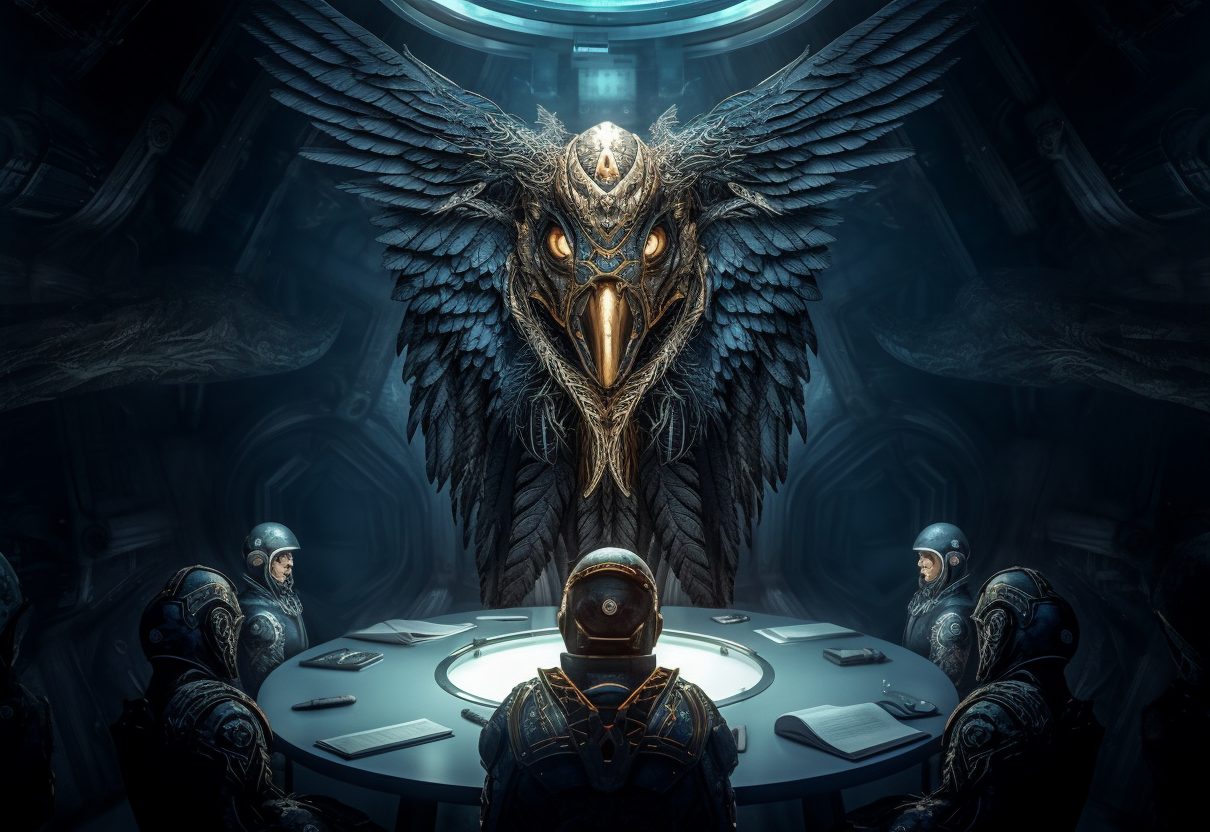
\includegraphics[width=0.48\textwidth]{chapter2_nyxi-meeting.png}
	\end{center}
	\caption{Don't be shy - grab a seat at the ambassador's table!}
\end{wrapfigure}

The inception of the ambassadorial role can be traced back to the initial
phases of the Human-Nyxi alliance. Recognizing the complexities inherent in
understanding and collaborating with an Nyxian entity, both species identified
the necessity for a liaison - someone steeped in the knowledge, customs, and
language of both worlds. Thus, the ambassador became the cornerstone of peace
and progressive dialogue.

Central to their role, ambassadors facilitate diplomatic communication between
Earth and Nyxophora. Tasked with maintaining and enhancing the amicable
relations between the two civilizations, they engage in policy discussions,
trade agreements, scientific collaborations, and more. Their adeptness at
interpreting the nuances of Nyxi communication ensures that messages don't get
lost or misconstrued in the void of space.

Another significant aspect of the ambassador's role is cultural mediation. They
are trained rigorously in Nyxi customs, art, history, and more, ensuring that
humanity can appreciate the richness of Nyxi society. Similarly, ambassadors
introduce the Nyxi to human cultural milestones, fostering mutual admiration
and understanding. Through this, both civilizations have been enriched, leading
to collaborative art projects, joint festivals, and shared educational
programs.

One of the paramount challenges during the early days of contact was linguistic
barriers. Today's ambassadors undergo years of immersive training in Nyxi
linguistics. Beyond just achieving basic comprehension of non-human
communication, fully understanding the Nyxi language's nuances, emotions, and
subtexts is pivotal. Ambassadors act as the prime interpreters during
high-level meetings, ensuring clarity and averting potential misunderstandings.

The ambassadorial role has proven paramount in fostering and maintaining the
flourishing relationship between humans and the Nyxi. As symbols of unity and
mutual respect, ambassadors ensure that the alliance remains not just on paper
but resonates deeply in the hearts and minds of both civilizations. The
intricate dance of cultures and languages is an ever-evolving journey.
Ambassadors, with their deep-rooted understanding of both worlds, will remain
instrumental in weaving the fabric of this joint destiny.

\section{Selection of Ambassadors}

Before embarking on the journey to become an ambassador to the Nyxi, one must
understand the depth of commitment and the magnitude of responsibility the role
entails. Ambassadors serve as living bridges, fostering unity, mutual respect,
and understanding; as such, the selection process is intricate and rigorous,
aiming to find individuals capable of thriving in this multifaceted role. The
Department of Ambassadorial Relations and Cosmosciences (DARC) is the official
worldwide institute that manages all certifications, from testing to training,
mission assignment and beyond.

Candidates aspiring to become ambassadors often come from diverse backgrounds,
including linguistics, interstellar diplomacy, cultural studies, and more.
However, a deep-seated interest in alien civilizations, particularly the Nyxi,
is paramount. Alongside academic and professional achievements, a potential
ambassador's emotional intelligence, adaptability, and resilience are
thoroughly assessed before any consideration.

DARC's testing phase involves a series of evaluations. Cognitive assessments
test an individual's ability to process complex information rapidly. Emotional
resilience is gauged through simulated interstellar situations, ensuring that
the candidate can maintain composure and rationality in high-pressure
scenarios. A panel, often comprising seasoned ambassadors, senior diplomats,
and Nyxi representatives, conducts in-depth interviews. These sessions
ascertain the candidate's motivations, depth of understanding of the role, and
their genuine interest in fostering human-Nyxi relations.

\subsection{General Requirements}

Once accepted to DARC, congratulations! You have now formally attained the
status of a `novant,' denoting your initiation into the ambassadorial cadre. A
diverse array of xenoacademic curricula awaits your selection. However, no
matter the path you decide, all novants have the same shared set of shared
requirements.

\subsubsection{Immersive Linguistic Training}
Learning the Nyx language goes far beyond mere vocabulary and syntax. Novants
immerse themselves in understanding the intricate dance of light and sound
inherent in Nyxi communication. Using advanced simulation technologies, they
experience Nyx linguistic patterns firsthand, mastering the nuances and
emotions embedded within, before moving on to producing the vast array of
phonemes required to communicate.

\subsubsection{Cultural Acclimatization}
Novants are submerged in Nyxi culture, history, art, and rituals. From
appreciating the ethereal Nyxi music to participating in their luminescent
festivals, trainees undergo a profound transformative experience, ensuring they
can represent human culture while deeply respecting and understanding the Nyxi.

\subsubsection{Diplomatic Etiquette and Protocol}
Given the critical nature of their role, novants are also trained in
interstellar diplomacy. They study treaties, understand protocols, and engage
in mock diplomatic scenarios, preparing them to handle urgent situations with
tact and grace.

\subsubsection{Real-world Experiences}
Before officially taking on the role, novants spend time on Nyx-Lystra,
engaging directly with the Nyxi. This final stage of training ensures that
theoretical knowledge is complemented by practical experience.

\subsection{Ambassadorial Specialization}
After completing the standard requirements, the next phase of training focuses
on a specialization. Each department at DARC offers a specific tailored
curriculum, guiding novants to the final stage of certified ambassador with a
unique expertise. The full listing of required courses is available in
\ref{Coursework}; here we will cover only the available specializations.

\begin{center}
	\textlbl{School of Engineering}
\end{center}

\subsubsection{Intergalactic Astronautics}
The Department of Intergalactic Astronautics offers a riveting journey from the
basics of spaceship design to the mastery of dark matter manipulation for warp
drives. Students incrementally build their expertise, moving from aeronautic
principles to cutting-edge materials, and then delve into specialized subjects
like quantum convolution and thermodynamics. Practical labs and projects in
each course deepen the students' understanding, while the capstone course on
emerging warp drive technologies bridges the scientific realms of both humans
and the Nyxi.

Astronauticists stand as the vanguard of human-Nyxi collaboration in the
intricate ballet of intergalactic travel. Specializing in spacecraft that can
navigate the Nyxi's home gas giant and exploit tenebrivity physics, these
professionals are key to humanity's forays into Nyxian territories. Their
skills enable them to retrofit Earth-based spacecraft with Nyxi dark matter
technology, facilitating safe and efficient intergalactic exchange. Through
their expertise, Astronauticists have even contributed to the co-design of
vessels capable of withstanding the multilayered forces in Nyx's complex
gaseous ecosystem.

\subsubsection{Xenobiological Engineering}
The Department of Xenobiological Engineering propels students through a
captivating curriculum that orbits the intersection of human biology and Nyxian
xenobiology. The courses escalate from foundational synthetic biology to
specialized subjects like nanoscale phenomena, tissue engineering, and
adaptomorphocytes. Hands-on labs, real-world challenges, and ethical debates
are a constant, culminating in an intricate understanding of Nyxian biology and
how it can harmonize with human engineering.

Xenobio Engineers operate at the enthralling confluence where human ingenuity
meets the mysterious biology of the Nyxi. Focusing on creating biologically
compatible machinery and therapeutics, these engineers are invaluable in
addressing Nyxian medical challenges that their advanced understanding of dark
matter can't resolve. Through the development of adaptomorphocytic cells and
bioauroraescence technology, Xenobio Engineers facilitate deeper biological
synchronization between Nyxi and human life. The role is not only technically
challenging but also ethically intricate, ensuring that collaborative ventures
respect the biological autonomy and intellectual heritage of both species.

\subsubsection{Tenebrichemical Engineering}
The specialization in Tenebrichemical Engineering offers an unparalleled
educational adventure into the mysterious realm of tenebrivity — the fifth
fundamental force tethered to dark matter. Beginning with a foundational
understanding of tenebrivity's theory and applications, students advance
through specialized courses on thermombranics, zophomaterial properties, and
propulsoskotic systems. Intriguing courses on metabolic engineering and
xenobiochemical processes illuminate the crossroads between tenebrivity and
xenobiology. The curriculum culminates in an ambitious exploration of Type IV
Kardashev Scale Sustainable Energy, setting the stage for engineering marvels
yet to come.

Tenebrichem Engineers are the architects of humanity's most audacious
collaborations with the Nyxi, pushing the boundaries of sustainable energy and
intergalactic travel. By harnessing tenebrivity, they unlock uncharted
engineering solutions that facilitate a myriad of possibilities — from crafting
next-generation propulsion systems to spearheading groundbreaking sustainable
energy projects. Tenebrichem Engineers are instrumental in translating Nyxian
chemistry and physics into human-compatible technologies, often working in
tandem with Nyxi scholars to create hybrid innovations. In doing so, they bring
humanity closer to the unimaginable — a civilization capable of Type IV
Kardashev Scale Sustainable Energy, advancing both human and Nyxi societies
into a new epoch of cosmic coexistence.

\subsubsection{Superluminal and Interstellar Engineering}
The Superluminal and Interstellar Engineering propels students into the
ethereal realms of warp drives and faster-than-light (FTL) travel. The
curriculum commences with the basics of Alcubierre theory and swiftly graduates
to the cutting-edge material science and ethics governing warp technology.
Amidst computer simulations and high-energy labs, students engage in capstone
projects that bring their theoretical warp drives to near-reality.
Supplementary modules on life support systems, Nyxian environments, and
interstellar traffic control enrich their multidimensional engineering prowess.

As Superluminalists, these experts become the fulcrum of human-Nyxi relations
in the realms of interstellar travel and colonization. Their mastery over warp
drive technologies allows humanity to venture into Nyxian territories, laying
the foundation for symbiotic explorations and joint scientific endeavors.
Skilled in creating and navigating the pathways of the cosmos, Superluminalists
facilitate quicker, ethical, and safer FTL journeys, often incorporating Nyxi
Tenebrivity principles for improved efficiency. These individuals are paramount
to the vision of an interwoven fabric of intergalactic civilizations, offering
an indispensable bridge between human aspirations and Nyxi scientific prowess.

\subsubsection{Xenophonologic Production}
Within the Department of Xenophonologic Production, students become the
polyglots of interstellar communication. Starting with the unique consonants
and triple-pitch vocalizations of the Nyxi, learners advance to mastering
auroral communication, blending sound and light into a symphony of transcendent
expression. Through the creative medium of neural networks and quantum
simulations, students become adept at synthesizing new auroral emitters and
neural interfaces. The department capitalizes on an interdisciplinary approach,
integrating elements from chaos theory to neural compatibility, often taught by
Nyxi experts via subspace links.

Xenophonologists serve as the voice in the delicate communion between humans
and Nyxi. Fluent in the multidimensional intricacies of Nyxi vocal-auroral
languages, they are key figures in crafting diplomatic channels and
facilitating groundbreaking scientific exchanges. Their skill in auroral-sonic
patterns enables them to convey abstract human concepts in a form the Nyxi can
easily grasp, and likewise, to interpret Nyxi information for human
understanding. Equipped with neural interfaces and custom-built auroral
emitters, Xenophonologists bridge cultural and scientific gaps, engendering an
unparalleled level of collaboration and mutual enrichment.

\subsubsection{Contraparadoxical Engineering}
In the enigmatic realm of Contraparadoxical Engineering, students embark on a
tantalizing journey from mastering quantum paradox prevention to dissecting the
chronostability of time travel. They'll then dabble in the alchemy of crafting
resilient extradimensional portals and demystify the holographic-virtual
reality intersection. By tackling the conundrums of recursive systems, the
coursework culminates in a philosophical contemplation of the ethics and
societal impacts of paradox-proof technologies.

Contraparadoxilists are the elite guardians of reality's fabric, ensuring
time-travel escapades and quantum endeavors don't result in catastrophic faux
pas. Their work's grandeur lies in crafting stable bridges between realms,
paramount for seamless human-Nyxi collaborations. With an unparalleled knack
for anticipating paradoxical pitfalls, they not only uphold the cosmic order
but thoughtfully ponder the societal ripples of their innovations. Their ethos?
Progress, yes, but never at reality's peril.

\subsubsection{Exotic Matter Science and Engineering}
Students of Exotic Matter Science and Engineering embark on a scintillating
journey to decode the enigma of unconventional forms of matter and energy.
Starting with an exploration of negative masses and tachyons, the curriculum
advances to the practical aspects of warp drives and wormhole stabilization.
Topics grow increasingly daring, covering everything from the computational
wonders of exotic matter states to the audacious concept of black hole power
plants. An indispensable ethics course ensures that students consider the
profound responsibilities that come with wielding such arcane knowledge.

Exoticists are the alchemists of the cosmos, crucially positioned at the
intersection between our understanding of the Nyxi's mastery of dark matter and
human expertise in exotic matter. Harnessing arcane forms of energy, they
facilitate the mind-bending technologies required for warp drives, a
pre-requisite for any interstellar rendezvous with the Nyxi. Their insights
into the stabilization of wormholes provide a direct gateway to Nyx, thus
amplifying the possibilities of intercultural exchange. Equipped with an
ethical compass, Exoticists navigate the turbulent waters of this high-stakes
science, ensuring that the pursuit of the unknown serves the collective
advancement of both civilizations.

\subsubsection{Vermiforamenic Medical Engineering}
Students in the Vermiforamenic Medical Engineering Department embark on an
exhilarating academic voyage through the arcane art of wormhole-mediated
medicine. Beginning with fundamental principles of vermiforamenology, the
course rapidly escalates into the integration of Nyxian spacetime manipulation
techniques for non-invasive surgeries. With a particular focus on ethical
considerations, students gain hands-on experience in optimizing imaging
systems, automating interventions, and experimenting with avant-garde concepts.
The curriculum culminates in speculative projects that dare to redefine the
boundaries of medical science. Note that this expertise is simply in the domain
of engineering. Those who wish to become a V-MD (Doctor of Vermiforamenic
Medicine) go on to join a 9-year medical school program.

Vermiforamenic Engineers operate at the edge of imagination and practicality,
functioning as the experts of non-invasive medical technology in collaboration
with the Nyxi. Harnessing the Nyxian mastery of tenebrivity to manipulate
microscopic wormholes, these engineers help revolutionize surgical
interventions, effectively reducing risks and expediting recovery times. Their
innovations in targeted drug delivery and remote medical care extend the
frontiers of both human and Nyxi healthcare. Working within stringent ethical
parameters, they ensure that this bold intersection of physics and medicine
remains a safe haven for transformative healing.

\begin{center}
	\textlbl{School of Expatriation}
\end{center}

\subsubsection{Enviroadaptive Habitation}
Within the Enviroadaptive Habitation Department, students explore the
intricacies of habitats that are as dynamic as the worlds they occupy. The
curriculum commences with an analysis of core technologies that enable habitats
to adjust to environmental flux. Students then engineer self-repairing
structures and adaptive microclimates, amalgamating urban design with natural
ecosystems for optimal sustainability. In a nod to closed-loop principles, the
coursework concludes with strategies to transmute waste products into essential
resources.

Enviroadaptists function as the architects of coexistence between humanity and
the enigmatic ecology of Nyx. By utilizing Nyxi advancements in Tenebrivity,
these specialists construct habitats that not only withstand the gas giant's
volatile environmental conditions but adapt and flourish within them. Their
pioneering work in microclimates and waste conversion serves as a conduit for
seamless human-Nyxi interaction, offering comfort and utility for both species.
Ultimately, Enviroadaptists pave the way for symbiotic colonization, converting
the alien landscapes into welcoming nexuses of shared existence.

\subsubsection{Nyxian Architecture}
Students in the Nyxian Architecture Department are submerged into the abstract
geometries and transformative qualities of Nyxi spatial design. The curriculum
begins with an examination of the Nyxi's unique perception of space and
function. Progressing through the program, scholars explore how Nyxian
structures are fluid, dynamic, and intrinsically resonant with their
surroundings while still maintaining a sense of fixed place. The academic
journey culminates in an intensive study of the Nyxi's urban planning, merging
architectural design with the very essence of their gaseous world.

Architectural Expatriatists are the creative diplomats in the shared domain of
Nyxian and human habitation. They interpret the complex geometries of Nyxian
design, seamlessly melding them with human architectural sensibilities. Their
deep understanding of sound and vibration in Nyxian structures allows for the
integration of Nyxi auroral communication within the built environment. It is
this fusion of Nyxian and human elements that makes Architectural Expatriatists
critical to crafting spaces where both species can collaborate, converse, and
thrive.

\subsubsection{Nyxian Sociology}
In the coursework of Nyxian Sociology, students embark on a labyrinthine
journey into the communal and individualistic facets of Nyxian culture.
Starting with foundational courses on societal norms and structures, scholars
unravel the rich tapestry of multilayered consciousness among the Nyxi. The
curriculum escalates to a rigorous study of Nyxian societal roles, rituals, and
the high-stakes arena of Nyxian arts. The academic odyssey concludes with an
analysis of Nyxi interspecies diplomacy, providing a multi-faceted view of
Nyxian social frameworks.

Sociologic Expatriatists serve as the cultural interpreters and mediators
between Nyxi and human societies. They deconstruct the complexities of Nyxian
societal norms and rituals, making them accessible to human understanding.
Their in-depth analysis of the Nyxi's multilayered consciousness offers new
paradigms for human-Nyxi collaborations, even shaping the ethics that govern
these interactions. Through the Sociologic Expatriatists' expertise, mutual
understanding flourishes, allowing for diplomatic and social exchanges that are
both meaningful and transformative for both species.

\subsubsection{Exonutrimental Gastronomy}
The Exonutrimental Gastronomy Department offers a gustatory journey through the
cosmos, with a special emphasis on Nyxian ingredients. Beginning with a
foundational overview of Nyxian gastronomic practices, students progress to
mastering intricate cooking techniques specific to extraterrestrial edibles. As
they gain proficiency, scholars explore the sensory richness of Nyxian foods,
from texture to triple-taste dimensions. The curriculum culminates in a
rigorous analysis of health impacts and the molecular ballet that these unique
ingredients undergo during culinary preparation.

Exonutrimental Gastronomicists stand at the tantalizing intersection of
culinary art and interstellar collaboration. Their expertise in preparing and
understanding Nyxian foods opens a new culinary frontier, acting as a
gastronomic bridge between species. By delineating the health benefits and
potential risks, they contribute to ethical food sourcing and consumption
practices. These gastronomicists are often invited to Nyxian feasts and events,
where they represent the epitome of human culinary achievement, thus
strengthening the social bonds between humans and the Nyxi.

\subsubsection{Exoplanetary Geography and Climate Acclimatization}
The Exoplanetary Geography and Climate Acclimatization program has students
embark on a fascinating tour of the universe's diverse terrains and climates.
The curriculum starts with a comprehensive look at landscapes and weather
patterns across known exoplanets. Students then engage in evaluating the
biological and technological adjustments required for human existence in these
alien climates. The coursework culminates in the study of exoplanetary liquid
systems and the impact of weather conditions on infrastructural designs.

The Exoplanetary Geographer performs an invaluable function in humanity's quest
to cohabit and collaborate with the Nyxi. With a meticulous understanding of
how terrains and climates interact on exoplanets, these geographers offer
guidance for the planning and establishment of sustainable projects, including
those on the Nyxi's gas-giant homeworld. By understanding the intricacies of
weather systems, they play a pivotal role in ensuring the success of
collaborative endeavors in unfamiliar environments. Their analyses often serve
as the backbone of diplomatic and exploratory missions, offering a grounded
context within which other scientific and cultural exchanges can occur.

\begin{center}
	\textlbl{School of Nyx Relations}
\end{center}

\subsubsection{Intergalactic Economics}
Students in the Intergalactic Economics Department find themselves amidst the
pulsating core of cosmic trade dynamics. Beginning with the elemental
principles governing galaxy-to-galaxy trade, the curriculum advances to the
labyrinthine monetary systems of various intergalactic civilizations. A nuanced
understanding of the logistics in trans-galactic good transfers follows. The
coursework culminates with an intimate examination of Nyxian economic practices
and the ethereal value of resources extracted from stars.

The Economic Nyxidocrat holds a crucial role in orchestrating and optimizing
the mutually beneficial trade between Earth and Nyx. Understanding the Nyxi's
unique valuation of dark matter and their application of Tenebrivity ensures
that humans can offer exchanges that are compelling to the Nyxi. By adeptly
navigating the complexities of galactic trade routes and policies, they
facilitate the smooth flow of goods, particularly in the arena of biology and
medicine where humans have a comparative advantage. Through their expertise,
they contribute to the ethical and sustainable proliferation of resources
between the two civilizations.

\subsubsection{Nyxtory}
Nyxian History offers a riveting chronicle through the evolution of Nyxi
civilization. The journey commences with the antiquity of Nyx, unfurling the
intricate tapestry of their ancient cultures and scientific triumphs. Students
then scrutinize the Nyxi's involvement in pivotal cosmic conflicts after
intergalactic colonization, a stage that sets the scene for exploring recent
societal transformations. Finally, the coursework examines the Nyxi's
labyrinthine foreign policies and cosmic alliances.

The Historical Nyxidocrat serves as a lynchpin for enriching human-Nyxi
collaboration through profound historical awareness. Understanding the deep
roots of Nyxi civilization and their ethical constructs, notably in the realm
of Tenebrivity, enables humans to establish more informed and respectful
dialogues. Their grasp of past Nyxi cosmic alliances and conflicts also
provides crucial context for shaping future intergalactic diplomatic
engagements. Essentially, the Historical Nyxidocrat acts as a temporal guide,
helping both species to navigate the complexities of their shared and separate
histories for a more harmonious future.

\subsubsection{Xenolinguistics}
The Xenolinguistics Department provides a comprehensive pedagogy of Nyxian
language and communication. Students begin with the foundational mechanics of
Nyxi vocal and auroral articulation, graduating to complex sentence formations
and semantic nuances. A series of courses explore everything from cultural
contexts to the cutting-edge technologies that facilitate Nyxi-human
communication. The final stretch of this linguistic marathon probes into
specialized arenas, including diplomatic language use and educational
methodologies, rounding off an exhaustive mastery of Nyxian linguistics.

The Xenolinguistic Nyxidocrat is the linchpin of cross-species communication,
navigating the subtleties of Nyxi communication. This mastery allows for more
authentic and nuanced dialogues, opening doors to advanced collaborative
ventures in fields like tenebrivity, art, and diplomacy. With a deep
understanding of Nyxi cultural cues and taboos, they prevent misunderstandings
that could otherwise set back intergalactic relations. They are not merely
translators, but architects of a shared linguistic space where Nyxi and humans
can coexist, collaborate, and enrich each other's understanding of the
universe.

\subsubsection{Nyxi-Human Relations}
Specializing in Nyxi-Human Relations offers students a deep understanding of
human-Nyxi interactions. From an in-depth dissection of our first fateful
meeting to an analytical survey of ongoing collaborative endeavors, the courses
weave together history, politics, and culture. Particular attention is paid to
the nuanced dance of diplomacy — exploring both triumphs in mutual
understanding and lessons learned from missteps. By the end of this
multidisciplinary adventure, students will be well-versed in the intricate
dynamics that govern this intergalactic relationship.

The Diplomatic Nyxidocrat stands as a beacon of interspecies partnership,
working tirelessly to forge sustainable connections between human and Nyxi
civilizations. These diplomats are not merely advisors, but creators of a
shared political and ethical lexicon that transcends both species. Skilled in
crisis management, they are able to diplomatically navigate misunderstandings
and controversies that could risk these tenuous ties. Equipped with a
comprehensive understanding of the subtleties of both human and Nyxi cultures,
Diplomatic Nyxidocrats play an essential role in negotiating the ethical and
political landscapes for cooperative ventures, from tenebrivity research to
medical exchange.

\subsubsection{Extraterrestrial Ethics and Philosophy}
The Department of Extraterrestrial Ethics and Philosophy offers an intellectual
view of Nyxian society and its philosophical underpinnings. Beginning with a
study of Nyxian ethical foundations, students progress to compare moral
philosophies across cosmic civilizations, employing case studies to sharpen
their ethical acumen. Deeper layers of complexity unfold as the coursework
dives into metaethical discussions and existential questions that span both
human and Nyxian perspectives. Ultimately, students emerge with a nuanced
understanding of morality in a cosmos teeming with life.

A Nyxidocratic Ethicist serves as an indispensable moral compass in the
complexity of interspecies interaction. Navigating divergent ethical frameworks
and moral imperatives, these ethicists mediate cultural clashes, finding common
ground where seemingly none exists. Their work is paramount in establishing
fair and ethical interstellar trade, diplomatic protocols, and collaborative
projects. Within the mosaic of ethical systems that arise in a universe that we
now know has sentient beings, Nyxidocratic Ethicists contribute to forging a
harmonious balance that benefits all involved.

\subsubsection{Cosmic Extradition and Law}
Students in Cosmic Extradition and Law embark on a rigorous exploration of
multi-galactic jurisprudence. The journey commences with learning the
fundamental principles that underpin celestial legal systems before wading into
the complexities of Nyxi-human extradition treaties and sentient rights. The
curriculum also unpacks the legal fabric of intergalactic commerce and outlines
the scaffolding of interstellar dispute resolution.

The Nyxidocratic Arbitrator serves as a lynchpin in navigating the intricate
lattice of legal systems that span human and Nyxi civilizations. Equipped with
an understanding of both species' legal traditions and intricacies, the
Arbitrator plays a vital role in crafting fair and enforceable treaties,
particularly in areas of extradition and trade. Their expertise in celestial
law is instrumental in averting or settling disputes that could escalate into
interstellar incidents. Consequently, the Arbitrator emerges as a bulwark
safeguarding mutual interests and fostering an atmosphere of cosmic harmony.

\subsubsection{Intersentiental Psychology and Behavior}
Intersentiental Psychology and Behavior encompasses an expertise in the
cognitive machinations common and unique to sentient life. From the multi-hued
spectrum of emotions, notably the Nyxi's auroral expressions, to the social
scaffolds of Nyxian communities, the coursework is comprehensive. One course
even offers a window into the rarely-discussed topic of interstellar mental
health. The capstone brings students face-to-face with the psychological
hurdles and biases that mar interactions between species, aiming for
enlightenment.

The Nyxidocratic Psychologist occupies a vital nexus in interstellar relations,
pioneering in the field where neuroscience meets diplomacy. By discerning the
psychological frameworks and social constructs of the Nyxi, they contribute to
the nuance and depth of inter-species dialogues. The role is particularly
significant in addressing any mental health concerns or societal issues that
arise in Nyxian civilizations, leveraging human advancements in psychology for
mutual benefit. Therefore, they not only unravel the enigmas of Nyxian thought
but also serve as architects of interspecies empathy.

\begin{center}
	\textlbl{School of Sciences}
\end{center}

\subsubsection{Physics of Tenebrivity and Aliquantics}
Within the Physics of Tenebrivity and Aliquantics department, students begin by
grounding themselves in the rudiments of dark matter physics and tenebrive
forces. As they advance, they navigate through the nebulous landscape of
non-standardized particles, thermodynamics under dark matter influences, and
quantum realms shaped by aliquant particles. The curriculum culminates in
aspirational courses that seek to unify the fragmented vistas of physics under
aliquantic principles, and explore the universe's grand tapestry through this
unique lens.

The Aliquantical Physicist stands at the cutting-edge intersection of Nyxian
and human physics. This role is quintessential for dissecting and understanding
the Nyxi's mastery of dark matter, tenebrivity, and thereby fostering
collaborative projects in intergalactic colonization and spacetime
manipulation. Through the elucidation of aliquantic principles, they demystify
the anomalies of Nyxian technologies, enriching both species with advanced
theories and applications. Consequently, their work functions as the
cornerstone upon which interstellar synergies in science are established.

\subsubsection{Xenobiology and Nebugenomics}
In the department of Xenobiology and Nebugenomics, students embark on an
intellectual voyage through Nyxian biodiversity and beyond. Beginning with
classifications based on morphological and genetic traits, learners transition
into intricate topics like Nyxian mutation rates and unique immune responses.
Advanced courses provide hands-on experience in alien genetic engineering and
delve into the ethics of xenobiological conservation. The curriculum culminates
in holistic examinations of life distribution across star systems, woven
together with computational genomics.

The Xenobiologist plays an indispensable role in the unfolding story of
human-Nyxi relations. Specialized in the biological makeup uniquely exhibited
by Nyxian species, they act as scientific ambassadors to decode the Nyxi's
complex organic, metallic, and ivory-based physiology. Their insights into
Nyxian ecological systems, immune responses, and genetics inform medical
collaborations and open up biotechnological frontiers. Moreover, their ethical
guidance in conservation and genetic manipulation ensures that the amalgamation
of Earth's biology with Nyxi nebugenomics proceeds in an equitable manner.

\subsubsection{Exoneuroscience and Polyphrenic Consciousness}
Within the Exoneuroscience and Polyphrenic Consciousness department, students
explore the fascinating realm of Nyxian neural configurations and thought
processes. The curriculum starts with an introduction to Nyxian polyphrenic
consciousness, advancing to comparative studies of neural pathways across
interstellar species. Students experiment with natural and artificial
substances that influence Nyxian cognition while also contemplating the ethical
implications of such interactions. Towards the end, learners plunge into the
mysterious world of Nyxian dreams and potential communication pathways between
human and alien neural systems.

A Polyphrenologic Exoneuroscientist operates at the intersection of science and
ethics, elucidating the enigmatic polyphrenic consciousness native to Nyxi
beings. They form the intellectual bridge that enables meaningful mental and
emotional exchanges between Nyxi and human species. By deciphering unique
Nyxian signaling pathways and neurotransmitter systems, these scientists pave
the way for cognitive enhancements and medical collaborations. Their in-depth
understanding of the ethics concerning exoneural interactions ensures that
humanity treads respectfully within the complex tapestry of Nyxian
consciousness.

\subsubsection{Galactostructural and Exoplanetary Sciences}
In the field Galactostructural and Exoplanetary Sciences, students join the
ongoing efforts to understand cosmic architectures and celestial phenomena.
Early courses lay the groundwork, delving into the geophysical properties of
exoplanets and the architectural intricacies of galaxies. As the curriculum
progresses, focus shifts towards deciphering multiplanetary fields, planetary
habitability, and even the cataclysmic ripples in tenebric spacetime. In the
latter stages, students confront ethically charged questions surrounding
terraforming and the search for extraterrestrial life signs.

A Galactostructuralist plays an instrumental role in understanding the Nyxi's
astral abode by studying the atmodynamics, pneumaphysics, and vortical
structuring of the gas giant Nyx. This invaluable knowledge not only paves the
way for human colonization efforts but also aids in mutually beneficial
resource-exchange programs with the Nyxi. Such professionals are often key
consultants when it comes to establishing artificial human habitats in Nyx,
ensuring both structural integrity and ethical viability. By studying phenomena
like Nyx's magnetic fields, Galactostructuralists also contribute to enhancing
auroral communication technologies between the Nyxi and humans.

\subsubsection{Novomathics and Transaxiomatic Computational Informatics}
Novomathics and Transaxiomatic Information Science has students undergo a
paradigm-shifting dive into the mathematical and computational universe of the
Nyxi. The curriculum begins with a foundational understanding of Nyxian
numbers, arithmetic, and geometric structures in higher dimensions. It
crescendos into the profound — exploring mathematics founded on alien axioms,
temporal paradoxes, and the enigmatic nuances of Nyxian logic. In advanced
stages, learners grapple with Nyxian systems of computation and the perplexing
hierarchies of Nyxian infinities.

The Novomathmetician stands as a crucial liaison in any collaborative venture
with the Nyxi, deciphering the mathematical principles that underlie their
technologies and philosophies. Armed with a deep understanding of Nyxian
numerical systems and computation, they facilitate efficient resource
allocation and technological integration between species. Their expertise in
curved spacetime mathematics makes them invaluable in mastering
tenebrivity-driven Nyxian warp drives. And as analysts of the Nyxi's unique
probabilistic models, Novomathmeticians also offer fresh insights into human
quantum mechanics and strategic decision-making processes.